\section{Tarea del 17 de septiembre de 2025}

\begin{ejercicio}
    Obtener la función masa de probabilidad conjunta de una m.a.s. de $X \rightsquigarrow B(k_0,p)$ y la función de densidad conjunta de una m.a.s. de $X \rightsquigarrow U(a,b)$.\\

    \begin{itemize}
        \item Consideramos $X \rightsquigarrow B(k_0,p)$\\
        
        Por definición tenemos que 
        \begin{gather*}
            P[X_1=x_1, \dots, X_n = x_n] = \prod_{i=1}^{n} P[X=x_i]\ \ \ ,(x_1, \dots,x_n) \in \chi^n 
        \end{gather*}
        Aplicándolo al caso particular de una distribución binomial tenemos que
        \begin{align*}
            P[X_1=x_1, \dots, X_n = x_n] &= \prod_{i=1}^{n} \binom{k_0}{x_i} p^{x_i} (1-p)^{(k_0-x_i)} = p^{\sum\limits_{i=1}^n x_i} \cdot (1-p)^{\sum\limits_{i=1}^n k_0 - x_i} \cdot \prod_{i=1}^{n} \binom{k_0}{x_i}
        \end{align*}

        \item Consideramos $X \rightsquigarrow U(a,b)$\\
        
        Por definición tenemos ahora que
        \begin{gather*}
            f_{(X_1,\dots,X_n)}(x_1,\dots,x_n) = \prod_{i=1}^n f_X(x_i)\ \ \ ,(x_1, \dots,x_n) \in \chi^n 
        \end{gather*}
        Conociendo la función de densidad de una distribución uniforme tenemos
        \begin{gather*}
            f_{(X_1,\dots,X_n)}(x_1,\dots,x_n) = \prod_{i=1}^n \frac{1}{b-a} = \frac{n}{b-a}
        \end{gather*}
    \end{itemize}
\end{ejercicio}

\begin{ejercicio}
    Dada una muestra aleatoria formada por las observaciones $(3, 8, 5, 4, 5)$, obtener su función de distribución muestral y realizar la representación gráfica.\\

    Por la definición de función de distribución muestral tenemos que
    \begin{align*}
        F^*_{X_1, \dots, X_5}(x) &= \frac{1}{5} \sum_{i=1}^5 I(-\infty,x](X_i) = \\
        &= \frac{1}{5} (I(-\infty,x](3) + I(-\infty,x](4) + 2I(-\infty,x](5) + I(-\infty,x](8))
    \end{align*}
    Lo que resulta 
    \begin{gather*}
        F^*_{X_1, \dots, X_5}(x) = \left\{
        \begin{array}{l l}
            \nicefrac{1}{5} \cdot 0 = 0 & \forall x \in (-\infty,3) \\
            \nicefrac{1}{5} \cdot 1 = \nicefrac{1}{5} & \forall x \in [3,4) \\
            \nicefrac{1}{5} \cdot (1+1) = \nicefrac{2}{5} & \forall x \in [4,5) \\
            \nicefrac{1}{5} \cdot (1+1+2) = \nicefrac{4}{5} & \forall x \in [5,8) \\
            \nicefrac{1}{5} \cdot (1+1+2+1) = \nicefrac{5}{5} = 1 & \forall x \in [8,\infty) \\
        \end{array}
        \right. 
    \end{gather*}

    Gráficamente resulta en:

    \begin{figure}[H]
    \centering
    \begin{tikzpicture}
        \begin{axis}[
            axis lines=left,
            height=6cm, width=14cm,
            xmin=-5, xmax=10,
            ymin=0, ymax=1.1,
            xtick={3,4,5,8},
            ytick={0,0.2,0.4,0.8,1},
            yticklabels={$0$,$\tfrac{1}{5}$,$\tfrac{2}{5}$,$\tfrac{4}{5}$,$1$},
            grid=major,
            axis x line=middle, % eje X en y=0
            axis y line=middle, % eje Y en x=0
        ]
            % Tramos constantes
            \addplot[very thick,red!60!black] coordinates {(-5,0) (3,0)};
            \addplot[very thick,red!60!black] coordinates {(3,0.2) (4,0.2)};
            \addplot[very thick,red!60!black] coordinates {(4,0.4) (5,0.4)};
            \addplot[very thick,red!60!black] coordinates {(5,0.8) (8,0.8)};
            \addplot[very thick,red!60!black] coordinates {(8,1) (10,1)};
            
            % Puntos abiertos y cerrados en los saltos
            \addplot[only marks,mark=o,red!60!black] coordinates {(3,0) (4,0.2) (5,0.4) (8,0.8)};
            \addplot[only marks,mark=*,red!60!black] coordinates {(3,0.2) (4,0.4) (5,0.8) (8,1)};
        \end{axis}
    \end{tikzpicture}
\end{figure}

\end{ejercicio}